\todo{Klassendiagramme erwähnen: Der Übersichtlichkeit halber einige getter/setter/toString,... weggelassen}

Nach der zuvor erstellen Konzeption folgt nun die Implementierung dieser Planungen. Im Fokus steht hier eine funktionale Umsetzung, welche praktisch aufzeigen soll, dass die erarbeiteten Konzepte auch praktisch umsetzbar sind. Es geht also nicht um seine umfangreiche oder perfekte Implementierung eines ganzen Slotbuchungssystems. Beide Optimierungsansätze werden dabei weiterhin getrennt voneinander, in zwei separaten Projekten umgesetzt. Auch die Beschreibung erfolgt deshalb nachfolgend in zwei getrennten Kapiteln.

\subsection{Entwicklungsumgebung und Projektaufbau}

Beide Projekte sind als normale Java Projekte, ohne besonders Framework aufgebaut. Sie nutzen die zum Zeitpunkt der Entwicklung aktuellste Version 22 von OpenJDK. Zur einfacheren Verwaltung der genutzten Libraries wird das Build-Werkzeug Maven eingesetzt. Genutzt werden in den Projekten jeweils zwei Libraries. Zum einen Lombok (in der Version 1.18.30), welche automatische Codegenerierung über Annotations ermöglicht und einfach dazu dienen soll, den Fokus auf den für dieses Projekt wesentlichen Code zu legen, indem die Generierung von Gettern, Settern und Konstruktoren ausgelagert wird. Für den Test der Algorithmen wird JUnit verwendet (Version 5.8.1). Dessen Zweck ist es, übersichtliche und strukturierte Testfälle für die Algorithmen aufzubauen. Da es keine Benutzeroberfläche und neben den Algorithmen auch kaum weiterreichende Kontrollstrukturen gibt, ist dies die beste Möglichkeit, die Algorithmen lauffähig zu machen.


\subsection{Algorithmus 1 (heuristische Ressourcenverteilung)}

Die hier niedergeschriebenen Kapitel sollen dazu dienen, die konkreten Gedanken und Details der durchgeführten Implementierung zu beschreiben. Dabei wird vor allem auf die Struktur, aber auch wichtige Daten und Abläufe eingegangen. Sehr spezifische Details zur exakten Implementierung und Funktionsweise des Codes werden hier eher nicht beschrieben, dies wurde an wichtigen und komplexen Stellen durch Kommentare im Code übernommen. Für das allgemeine Verständnis der Implementierung ist dies aber auch nicht entscheidend und eine rein textuelle Beschreibung von komplexen Codestellen würde das Verständnis auch nicht unbedingt fördern.

Die Implementierung gliedert sich in bedeutende und zusammenhängende Bestandteile, welche im Folgenden einzeln genauer erläutert werden.


\subsubsection{Aufbau und Entwurfsmuster}

\todo{Quelle MVC?!}

Da es sich hier um eine sehr grobe und prototypische Implementation der geplanten Algorithmen handelt, ergibt es kaum Sinn, besondere Entwurfsmuster o.ä. zu verwenden. Ohne eine umfangreiche Planung einer potentiellen gesamten Software ist es hier ohnehin kaum möglich ein perspektivisch dafür passendes Entwurfsmuster zu Grunde zu legen. Orientiert wurde sich bei diesem Projekt deshalb an dem einfachen Model-View-Controller (MVC) Prinzip. Das MVC hat den Vorteil, dass es Datenstrukturen, Kontrollstrukturen und die Präsentation der Daten trennt. So kann die Darstellung der Daten übersichtlich getrennt werden, was eine spätere Implementierung dieser Algorithmen in einen anderen Softwarekontext erleichtert, weil so schon klare Datenschnittstellen definiert sind. Die Kontrollstrukturen sind in diesem Fall die Algorithmen, welche ebenfalls getrennt und übersichtlich abgelegt werden. Eine richtige View, also Benutzeroberfläche gibt es in diesem Fall noch gar nicht. MVC wird aber häufig auch wegen seiner guten Austauschbarkeit der Präsentation der Daten eingesetzt. Somit wäre es hier später auch einfacher möglich, eine richtige Benutzeroberfläche anzusetzen.


\subsubsection{TruckAdvices}

Die Basis des Projekts bilden, wie bereits ausführlich herausgearbeitet wurde, die LKW Buchungen bzw. Avisierungen am Terminal. Um die entsprechenden Daten zu halten, wurde eine passende Datenstruktur aufgebaut. Das Hauptobjekt ist dabei TruckAdvice, welches die eigentliche Avisierung eines LKW enthält. Dies sind alle Daten, die von einer entsprechend vorgeschalteten Benutzeroberfläche erfasst werden müssen, um eine sinnvolle Verarbeitung und Planung der Aufträge durchführen zu können. Darunter sind einige Parameter, welche für den hier entwickelten Algorithmus unumgänglich sind. Dies sind numberOfGoods und die HandlingCategory. Alle weiteren Daten, wie Warentyp, Beschreibung, Buchungsnummer, Gewicht und Ausmaße sind für diese Implementierung nicht von besonderer Wichtigkeit, dennoch sind sie wichtige Angaben die im späteren Ladeprozess im Hafen vollständig und korrekt sein sollten, um eine gute Vorbereitung zu gewährleisten und Fehler zu vermeiden. Aus Gründen der Datenhaltung und der leichteren Verarbeitung wurde entschieden, die ausgewählte Zeit bzw. den Slot nicht direkt im Objekt zu speichern, sondern über eine entsprechende Liste pro Slot, denen jeweils die TruckAdvice Objekte hinzugefügt werden.

\begin{figure}[H]
    \centering
    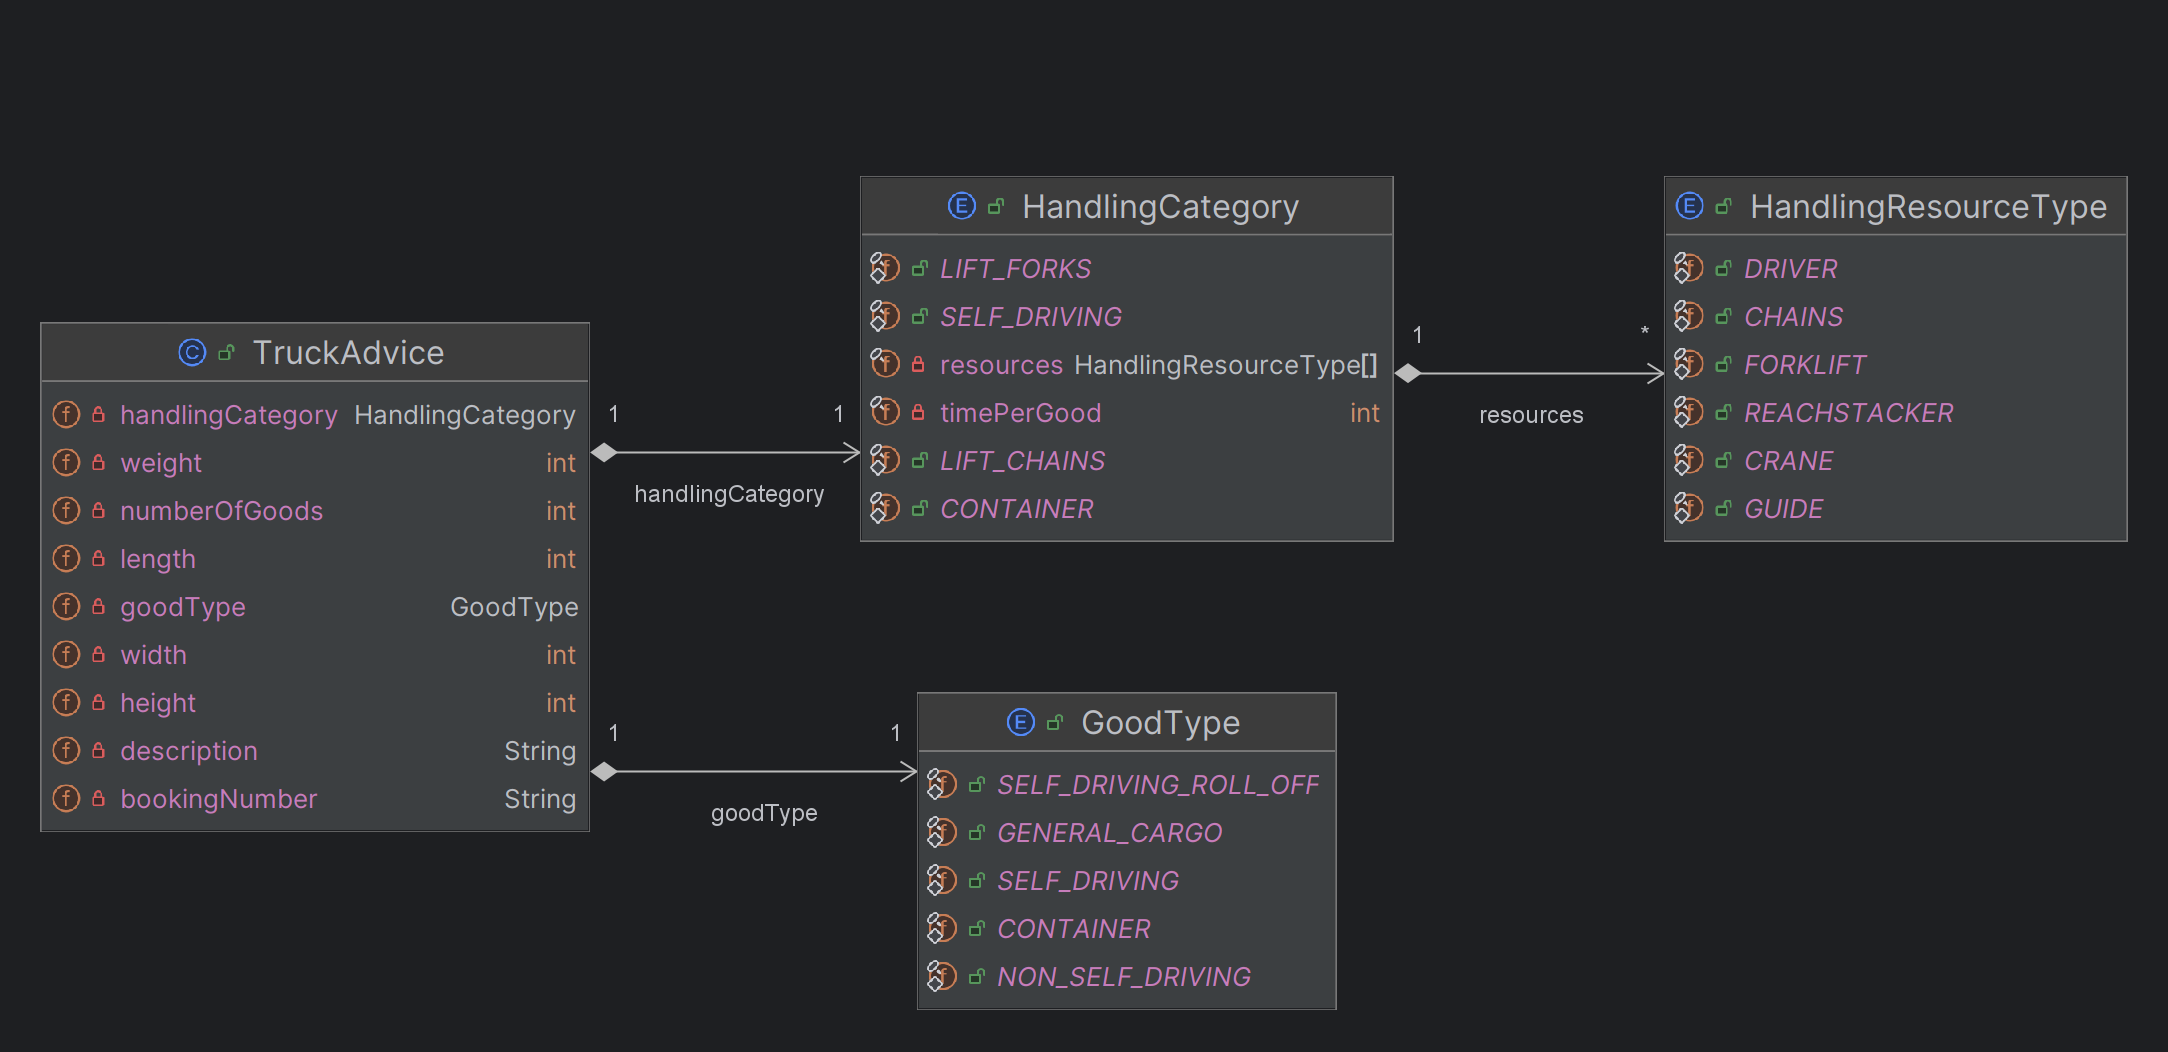
\includegraphics[width=\textwidth]{images/classDiagrams/TruckAdvice_ClassDiagram.png}
    \caption{Klassendiagramm der Modell-Klassen im Zusammenhang mit TruckAdvice}
    \label{fig:classDiagramTruckAdvice}
\end{figure}

Um eine Kategorisierung und eindeutige Bestimmung der gelieferten Güter zu ermöglichen, ohne Spielraum und Unklarheiten durch Freitextfelder zu erzeugen, wurden die wichtigsten Daten durch Enums erfasst. Diese erlauben auch eine spätere Anpassung oder Erweiterung der bisher vorgegebenen Daten. Bedeutender für die Planungsalgorithmen ist aber die HandlingCategory. Dies ist ein fester Satz von Arten, wie ein Gut abgeladen werden kann. Pro Kategorie kann hier eingestellt werden, wie lange es dauert, ein Gut dieses Typs vom LKW abzuladen. Außerdem kann eine Liste von Ressourcentypen (HandlingResourceType) angegeben werden, die zur Verarbeitung im Hafen nötig sind. Diese HandlingResourceTypes bilden die letzte Enum.

Alle Enums wurden mit Werten entsprechend der Analyse aus Kapitel \ref{sec:analyseAbfertigung} gefüllt. Folgende Werte sind dabei aktuell gesetzt, wobei Erweiterungen durch die Wahl des Typs Enum möglich sind, ohne umfangreichere Anpassungen vornehmen zu müssen: \todo{Enumwerte final?}

GoodType: CONTAINER, GENERAL\_CARGO, SELF\_DRIVING, SELF\_DRIVING\_ROLL\_OFF, NON\_SELF\_DRIVING

HandlingResourceTypes: FORKLIFT, CRANE, REACHSTACKER, GUIDE, DRIVER, CHAINS

HandlingCategory: 
\begin{itemize}
    \item LIFT\_CHAINS (timePerGood: 12, HandlingResourceTypes: CRANE, GUIDE, CHAINS)
    \item LIFT\_FORKS (timePerGood: 5, HandlingResourceTypes: DRIVER, GUIDE)
    \item SELF\_DRIVING (timePerGood: 8, HandlingResourceTypes: REACHSTACKER, CHAINS)
    \item CONTAINER (timePerGood: 8, HandlingResourceTypes: REACHSTACKER, CHAINS)
\end{itemize}



\subsubsection{Zeitplan}

Ein wesentlicher Bestandteil des hier gezeigten Ansatzes ist die Erstellung eines Zeitplans (Schedule). Um also Algorithmen zu entwickeln, welche einen Zeitplan erzeugen können, musste zunächst einmal eine passende Datenstruktur mit entsprechenden Kontrollstrukturen entwickelt werden. 

\begin{figure}[H]
    \centering
    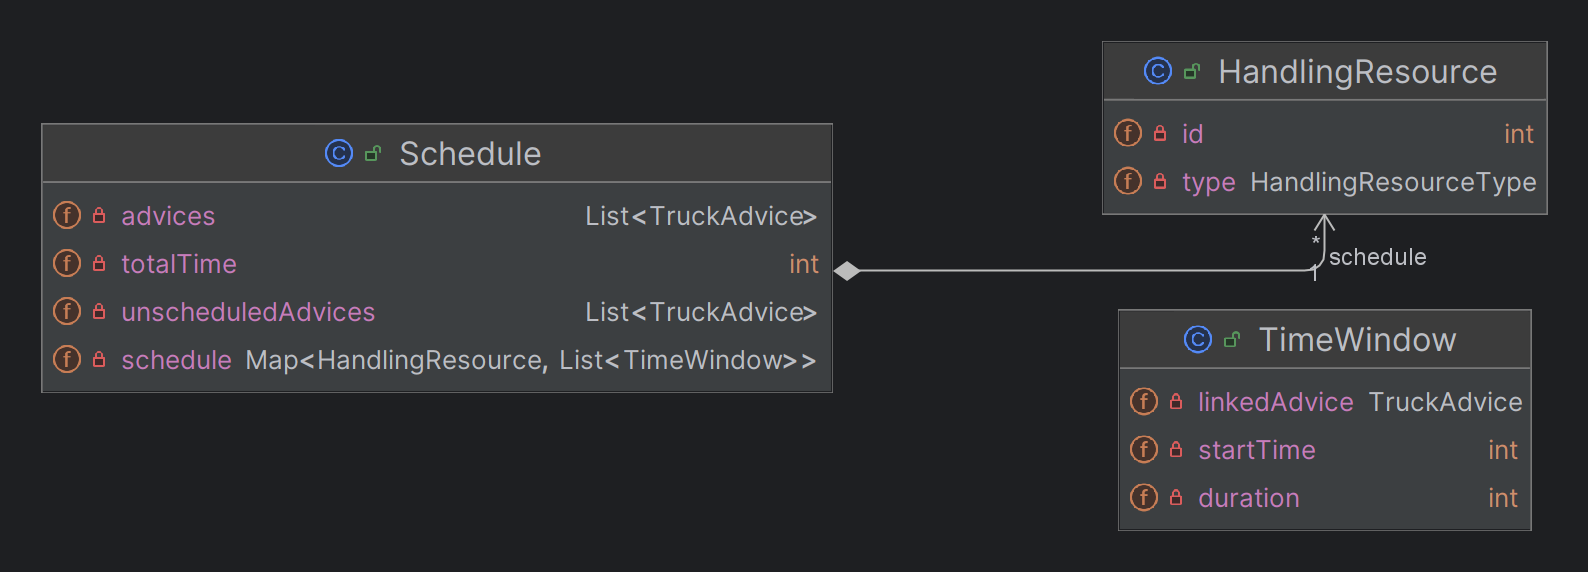
\includegraphics[width=\textwidth]{images/classDiagrams/Schedule_ClassDiagram.png}
    \caption{Klassendiagramm der Modelklassen im Zusammenhang mit Schedule}
    \label{fig:classDiagramSchedule}
\end{figure}

Grundidee ist, dass ein Zeitplan aus verschiedenen parallelen Zeitachsen für unterschiedliche Ressourcen besteht. Der gesamte Zeitplan hat dabei eine eindeutige Gesamtlänge in Minuten, um die Länge eines Zeitslots darzustellen. Es ist dabei so, dass jede Zeitachse durch Zeitfenster (TimeWindow) belegt werden kann. Diese können nur nacheinander liegen und haben jeweils einen Startzeitpunkt und eine Dauer in Minuten. Die Datenstruktur eines Schedules ist deshalb relativ einfach aufgebaut: Eine Map beinhaltet jeweils die verfügbaren Ressourcen als Key und ordnet jeder Ressource eine Liste von TimeWindows zu, in denen diese belegt ist. Die Liste der belegten Zeitfenster ist dabei immer nach Startzeit, also chronologisch sortiert. Um einen besseren Überblick über alle Avisierungen zu behalten und auch um alle noch nicht oder nicht mehr planbaren Avisierungen zu speichern, enthält ein Schedule Objekt jeweils eine Liste der entsprechenden TruckAdvices. 

Damit die Planungsalgorithmen mit einem Zeitplan arbeiten können, werden diverse, teils komplexere Abfragen und Operationen auf die Schedule Objekte benötigt. Um diese Operationen ohne Codedopplungen und separiert von dem Datenobjekt Schedule erreichbar zu machen, wurde dafür eine Klasse \textit{ScheduleUitls} angelegt. Alle Methoden sind dabei statisch, da sie auf einem übergebenen Schedule Objekt arbeiten und lediglich Abfragen darauf ausführen, ohne komplexere Daten halten zu müssen. Folgende Methoden sind verfügbar und können von allen Planungsalgorithmen genutzt werden:

\begin{itemize}
    \item \textit{findAvailableResourceByType(Schedule schedule, HandlingResourceType type, TimeWindow window): HandlingResource}

    Findet innerhalb des Zeitplans eine passende Ressource, die im angegebenen Zeitfenster verfügbar ist. Dies ist vor allem interessant, wenn nach der Suche von Zeitfenstern eine passende Ressource gebucht werden soll.    
    
    \item \textit {checkWindowsOverlapping(TimeWindow w1, TimeWindow w2): boolean}

    Prüft, ob zwei angegebene Zeitfenster zeitlich überlappen, d.h. ob sich diese zeitlich überschneiden oder ob sie einfach nacheinander gebucht werden können.
    
    \item \textit{findEmptyTimeWindows(Schedule schedule, HandlingResourceType resourceType): List\textless{}TimeWindow\textgreater{}}

    Diese Methode such alle verfügbaren Zeitfenster für einen bestimmten Ressourcen Typ innerhalb des Zeitplans. Dies ist vor allem interessant, um zu planen, wann freie Zeiträume für welche Avisierung verfügbar sind.
    
    \item \textit{getOverlappingWindows(Schedule schedule, List\textless{}TimeWindow\textgreater{} list1, List\textless{}TimeWindow\textgreater{} list2): List\textless{}TimeWindow\textgreater{}}

    Gibt eine Liste von Zeitfenstern zurück, in denen sich die Zeitfenster aus zwei separaten Listen überschneiden. Das ist vor allem interessant, um zu schauen, wann zwei oder mehr Ressourcen gleichzeitig verfügbar sind.
    
    \item \textit{cleanWindowList(List\textless{}TimeWindow\textgreater{} list): List\textless{}TimeWindow\textgreater{}}

    Entfernt alle Zeitfenster, die komplett in einem anderen enthalten sind. Es kann sonst möglicherweise zu Problemen kommen, wenn durch verschiedene Operationen keine saubere Liste erzeugt wurde, bei der alle Zeitfenster chronologisch und ohne Überschneidungen vorliegen.
    
    \item \textit{getBiggestWindow(List\textless{}TimeWindow\textgreater{} list): TimeWindow}

    Sucht das größtmögliche Zeitfenster aus einer übergebenen Liste heraus.
    
    \item \textit{getSmallestWindow(List\textless{}TimeWindow\textgreater{} list, int minTime): TimeWindow}

    Sucht das kleinstmögliche Zeitfenster aus einer übergebenen Liste heraus.
\end{itemize}

Viele der genannten Methoden sind durchaus komplex und bergen Fehlerpotenziale, insbesondere bei der Arbeit mit Zeitfenstern und deren Relationen zueinander. Innerhalb der eigentlichen Planungsalgorithmen werden allerdings viele der Methoden bereits intensiv eingesetzt, so konnten bereits viele Fehler durch manuelle Tests beseitigt werden.\todo{Zu einigen Methoden konnten auch automatisierte Testfälle zur Überprüfung geschrieben werden; Automatisierte Tests schreiben?} Aus Zeitgründen und einer Kosten-Nutzen-Abwägung wurde entschieden, dass dieser Aufwand und Umfang zur Fehlersuche ausreicht. Nach vielen manuellen Überprüfungen konnten schlussendlich keine Fehler mehr entdeckt werden, die Fehlerrate sollte also wenn überhaupt vorhanden, sehr gering sein.



\subsubsection{Planungsalgorithmen}

Die Implementierung der Algorithmen ist der zweite bedeutende Bestandteil bei der Entwicklung dieses Projekts. Wie in der Planung beschrieben, wurden mehrere Sortierungsverfahren parallel implementiert werden, um am Ende einen Vergleich anstellen zu können. Um eine möglichst gute Modularität, Austausch- und Erweiterbarkeit zu erzielen, wurde jeder Algorithmus in einer eigenen Klasse umgesetzt, welche von der abstrakten Hauptklasse \textit{Scheduler} erbt. Diese definiert eine feste Methode, welche einen Zeitplan für einen Zeitslot erzeugt, wenn sie eine Liste von gebuchten LKW, eine Liste der zu diesem Zeitpunkt im Terminal verfügbaren Ressourcen und die Länge des Zeitslots übergeben bekommt. Eingangs- und Ausgangsschnittstellen sind somit klar definiert und die Logik dazwischen kann beliebig ausgetauscht werden, auch zukünftig.

\begin{figure}[H]
    \centering
    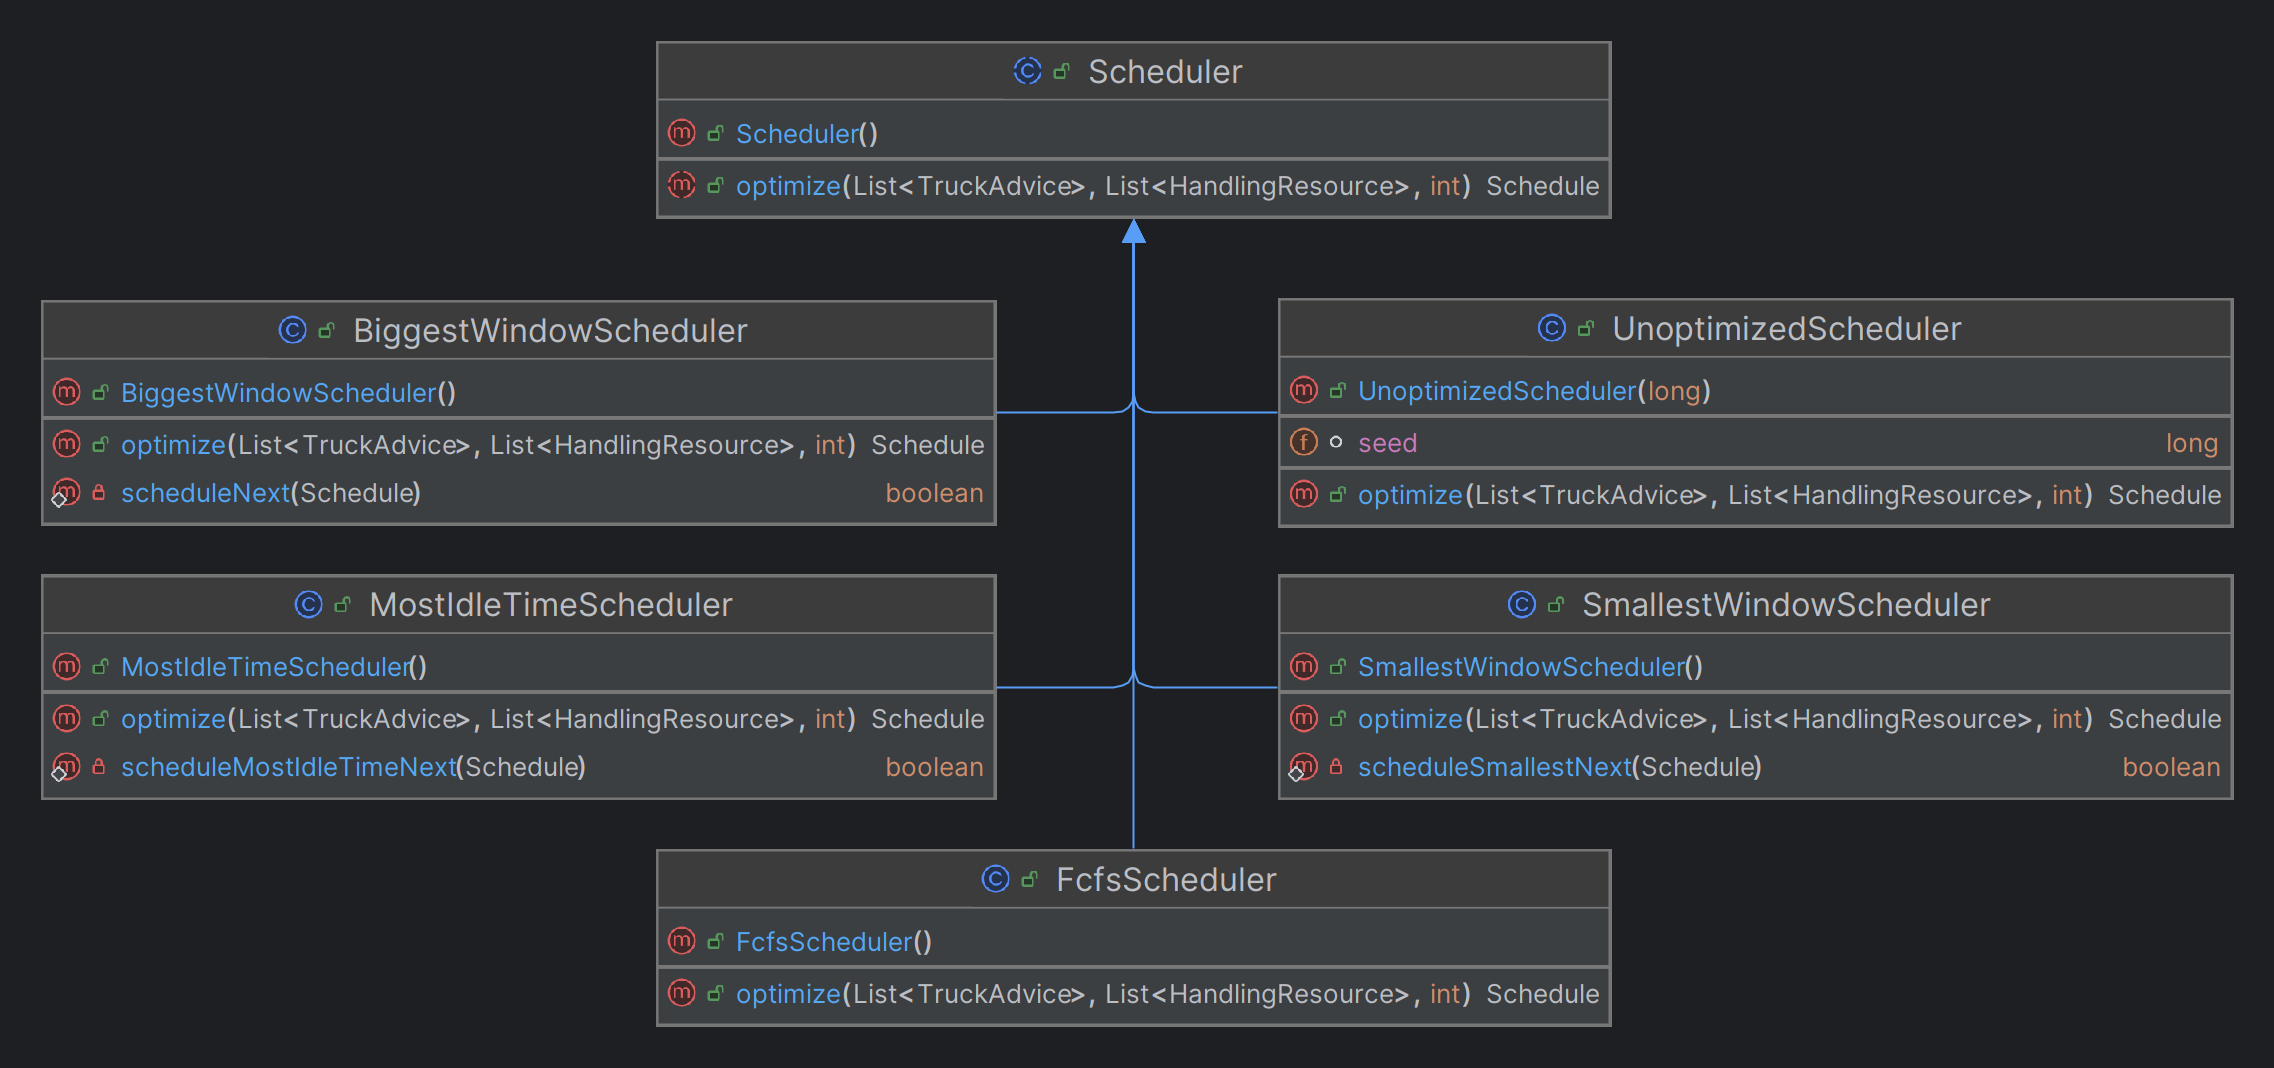
\includegraphics[width=0.7\textwidth]{images/classDiagrams/Scheduler_ClassDiagram.png}
    \caption{Klassendiagramm aller Controller-Klassen, die von Scheduler erben}
    \label{fig:classDiagramScheduler}
\end{figure}

Besonders hervorzuheben ist im Klassendiagramm (siehe Abb. \ref{fig:classDiagramScheduler}) die Klasse \textit{UnoptimizedScheduler}. Sie stellt die Implementierung der im Konzept in Kapitel \ref{sec:konzeptRsVergleichswerte} geplanten Generierung von Vergleichswerten dar. Um hier ebenfalls eine einfache Generierung mit gleichen Eingangs- und Ausgangsformaten und somit einem leichten direkten Vergleich zu erzielen, wurde dies ebenfalls weitere Subklasse von \textit{Scheduler} implementiert. Statt einer Optimierung wird hier einfach ein simulierter Zeitplan, wie er in der Konzeption beschrieben wurde, erzeugt und zurückgegeben. Bei der Entwicklung der Algorithmen wurde ansonsten darauf geachtet, soweit Zufallswerte eingesetzt wurden, diese mit der Möglichkeit auszustatten, Seeds zu übergeben. Dies soll die Wiederholbarkeit von späteren Testläufen sicherstellen. Im Praxiseinsatz kann hier einfach mit zufälligen Werten oder Standardseeds gearbeitet werden. Die genaue Implementierung der Algorithmen orientiert sich dabei sehr stark an der Planung auf Kapitel \ref{}\todo{Kapitelangabe}. Die genaue Funktionsweise lässt sich dabei sehr gu anhand der Kommentare in den jeweiligen Code-Klassen (siehe Abbildung \ref{fig:classDiagramScheduler}) nachvollziehen. Eine erneute Beschreibung wurde deshalb an dieser Stelle ausgespart.
\todo{- Algorithmen erklären? Noch mehr schreiben?!}


\subsubsection{Analyse der Zeitplanungen}

Alle nach den unterschiedlichen Verfahren erstellten Zeitpläne liegen nun in einem einheitlichen Format als \textit{Schedule}-Objekt vor. Dies ermöglicht auch eine über alle Verfahren einheitliche Auswertung. Um im Verlauf dieser Arbeit Analysen und eine Evaluation durchführen zu können, wurde aus diesem Grund eine eigene Controller-Klasse \textit{ScheduleAnalyser} erstellt, welche alle interessanten Werte aus dem \textit{Schedule} berechnet und als einheitliches \textit{ScheduleAnalysis}-Objekt speichert und zurück gibt. 

\begin{figure}[H]
    \centering
    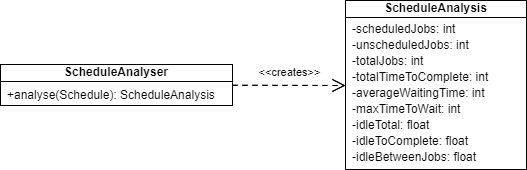
\includegraphics[width=0.9\textwidth]{images/classDiagrams/ScheduleAnalyser_ClassDiagram.png}
    \caption{Klassendiagramm von ScheduleAnalyser und der erzeugten ScheduleAnalysis}
    \label{fig:classDiagramScheduleAnalyser}
\end{figure}

Folgende Werte werden dabei berechnet:

\todo{Alle Attribute von ScheduleAnalysis auflisten, Rechenweg und Zweck erklären, Bilder zur Verdeutlichung hinzufügen?}

\begin{itemize}
    \item \textit{scheduledJobs:} Die Anzahl der LKW, die erfolgreich in den Zeitslot eingeplant werden konnten. Die Erhöhung dieses Wertes ist da Hauptziel der Optimierung, eine insgesamt effizientere Planung sollte am Ende dafür sorgen, dass mehr LKW innerhalb des gleichbleibenden Slots bearbeitet werden können.
    \item \textit{unscheduledJobs:} Die Anzahl von LKW, die zeitlich nicht mehr in den Slot gepasst haben.
    \item \textit{totalJobs:} Die Gesamtanzahl der avisierten LKW, welche versucht wurden, auf den Slot zu verteilen (entspricht scheduledJobs+unscheduledJobs).
    \item \textit{totalTimeToComplete:} Die Dauer in der innerhalb des Slots Ressourcen belegt werden. Dies ist vor allem interessant, um ein Maß für die Optimierung zu haben, wenn der Slot nicht komplett mit LKW ausgefüllt ist. Je schneller dann die Arbeit beendet ist, desto mehr können die Ressourcen an anderer Stelle eingesetzt werden.
    \item \textit{averageWaitingTime:} Die durchschnittliche Zeit von Beginn des Slots, bis zum Beginn der Bearbeitung eines LKW. 
    \item \textit{maxTimeToWait:} Die maximale Zeit, welche ein LKW seit Beginn des Slots warten muss, bis er abgeladen wird.
    \item \textit{idleTotal:} Die Summe der Leerlaufzeiten aller Ressourcen, in denen sie für keinen Jobs eingebunden sind.
    \item \textit{idleToComplete:} Die Summe der Leerlaufzeiten aller Ressourcen, bis alle Aufträge abgearbeitet sind. Ein relatives Maß, falls zu wenig LKW für den ganzen Slot vorhanden sind. Die Gesamtleerlaufzeit würde hier sehr stark nach oben gehen, obwohl Ressourcen dann evtl. ganz woanders eingesetzt werden könnten.
    \item \textit{idleBetweenJobs:} Die Summe der Leerlaufzeiten aller Ressourcen zwischen Aufträgen. Vor Beginn des ersten LKW und nach Ende des letzten LKW kann eine Ressource möglicherweise an anderer Stelle eingesetzt werden. Viele auseinander gezogene Jobs mit vielen kurzen Leerlaufzeiten zwischendurch sind unschön für eine optimale Auslastung.
\end{itemize}


\subsubsection{Grundlagen für JUnit Tests}

\todo{Generierungsklasse und CSV Exporter genauer erläutern?}

Um schlussendlich sinnvolle Testläufe und Auswertungen der implementierten Algorithmen durchführen zu können, wurde eine Basis für JUnit Tests geschaffen. Genaue Details zu den konkreten Testfällen und deren Implementierung finden sich jeweils an gegebener Stelle im nachfolgenden Evaluationskapitel oder in Kommentaren im Testcode. Es wurden allerdings einige Testübergreifende Grundlagen implementiert, welche hier schon einmal genauer erläutert werden.

Zum einen braucht es hier die Möglichkeit passende und realitätsnahe Eingangsdatensätze, also insbesondere Listen von TruckAdvices zu generieren. Dafür wurde eine entsprechende Methode in der Test-Klasse \textit{AdviceGenerator} geschrieben. Neben der Anzahl der Buchungen, also der Größe des zu generierenden Datensatzes erhält die Methode auch ein Array \textit{ratioPerCategory}. Hier kann eingestellt werden, wie das Verhältnis der Ladungskategorien in der generierten Liste sein soll. So kann entweder eine stärkere Ungleichverteilung, aber auch eine Anpassung an reale Verhältnisse erzeugt werden. Außerdem arbeitet die Methode mit Zufallswerten. Wie auch schon bei der Implementierung der Algorithmen erwähnt, ist es hier besonders wichtig, mit Seeds zu arbeiten, um wiederholbare Testläufe zu erzeugen. Aus diesem Grund enthält auch jeder Testfall zunächst ein Random-Objekt mit festgelegten Seed, aus dem in dieser Testmethode benötigten Werte generiert werden.

Der zweite wesentliche Bestandteil jedes Tests, ist der eigens entwickelte \textit{CsvExporter}. Diese Klasse ermöglicht es sehr einfach die Testreihen und Datensätze jedes Durchlaufs in entsprechende CSV-Dateien zu schreiben. CSV ist ein einfaches Format zur standardisierten und strukturierten Speicherung von Daten bzw. Datentabellen \cite{csvFormat}. So können die Daten zur weiteren Auswertung sehr einfach und ohne großen Aufwand in jedem Testfall gespeichert werden. Das CSV Format ist auch gut geeignet um es in R-Skripte zu importieren und weiterzuverarbeiten.



\subsection{Algorithmus 2 (Planung der Reihenfolge mit TSP)}

Von der grundsätzlichen Struktur und den Gedanken zum Aufbau unterscheidet sich die Implementierung dieses Algorithmus gar nicht stark von der zuvor beschriebenen Umsetzung des anderen Algorithmus. Aus diesem Grund hat auch der nachfolgende Aufbau der Beschreibung eine große Ähnlichkeit. Der Fokus wird hier deshalb auch konkreter auf spezielle Entscheidungen und Unterschiede gelegt, gemeinsame Entscheidungen werden hier nicht so tief erläutert und begründet. Dabei wird auch in dieser Ausführung mehr Fokus auf die Beschreibung der wichtigen Strukturen, Daten und Abläufe gelegt. Konkrete Beschreibungen von komplexen Codestellen, welche auch für das allgemeine Verständnis der Implementierung nicht so wichtig sind, werden wieder eher durch Kommentare im Code übernommen.

Die Implementierung lässt sich in einige Hauptbestandteile gliedern, welche in den folgenden Kapiteln genauer beschrieben werden.


\subsubsection{Aufbau und Entwurfsmuster}

Auch dieses Projekt wurde auf Basis des Model-View-Controller Musters aufgebaut. Denn auch an dieser Stelle ist die Trennung von Daten- und Kontrollstrukturen sehr sinnvoll, weil sich so die Datenobjekte und Schnittstellen gut von den eigentlichen Algorithmen trennen lassen. Auch wenn sie hier ebenfalls noch nicht implementiert wurde, lässt sich eine Benutzeroberfläche so später sehr einfach hinzufügen bzw. die Kontrollstrukturen in eine bestehende Oberfläche integrieren. 


\subsubsection{TruckAdvices}

Die Struktur des Datenmodells der LKW Avisierungen ähnelt auch sehr der Umsetzung des anderen Algorithmus. Die grundsätzlich gespeicherten und verarbeiteten Daten sind dabei aus Endnutzer Sicht im Hauptobjekt \textit{TruckAdvice} identisch. Der Unterschied ist in diesem Fall hauptsächlich die Implementierung der \textit{HandlingCategory}. Einer Kategorie ist dabei jeweils die benötigte Maschine zugewiesen, welche zum Be- oder Entladen des entsprechenden LKW benötigt wird. Eine \textit{HandlingMachine} ist wiederum charakterisiert durch die mit ihrer Nutzung verbundenen Zeitaufwände, also Aufbauzeit (setupTime), Ladezeit pro Gut (timePerGood) und Abbauzeit (endTime). Im Vergleich zu dem anderen Ansatz findet hier eine deutlich größere Abstraktion statt. Während im anderen Fall konkrete Ressourcen bekannt sind, steht in dieser Umsetzung jede Ressource stellvertretend für alle in diesem Zusammenhang benötigten weiteren Ressourcen, wie entsprechende Fahrer oder Einweiser etc. Hier wird der Fokus dafür mehr auf die Berechnung des Zeitaufwands gelegt, was in der anderen Implementierung nicht der Fall war. 

\begin{figure}[H]
    \centering
    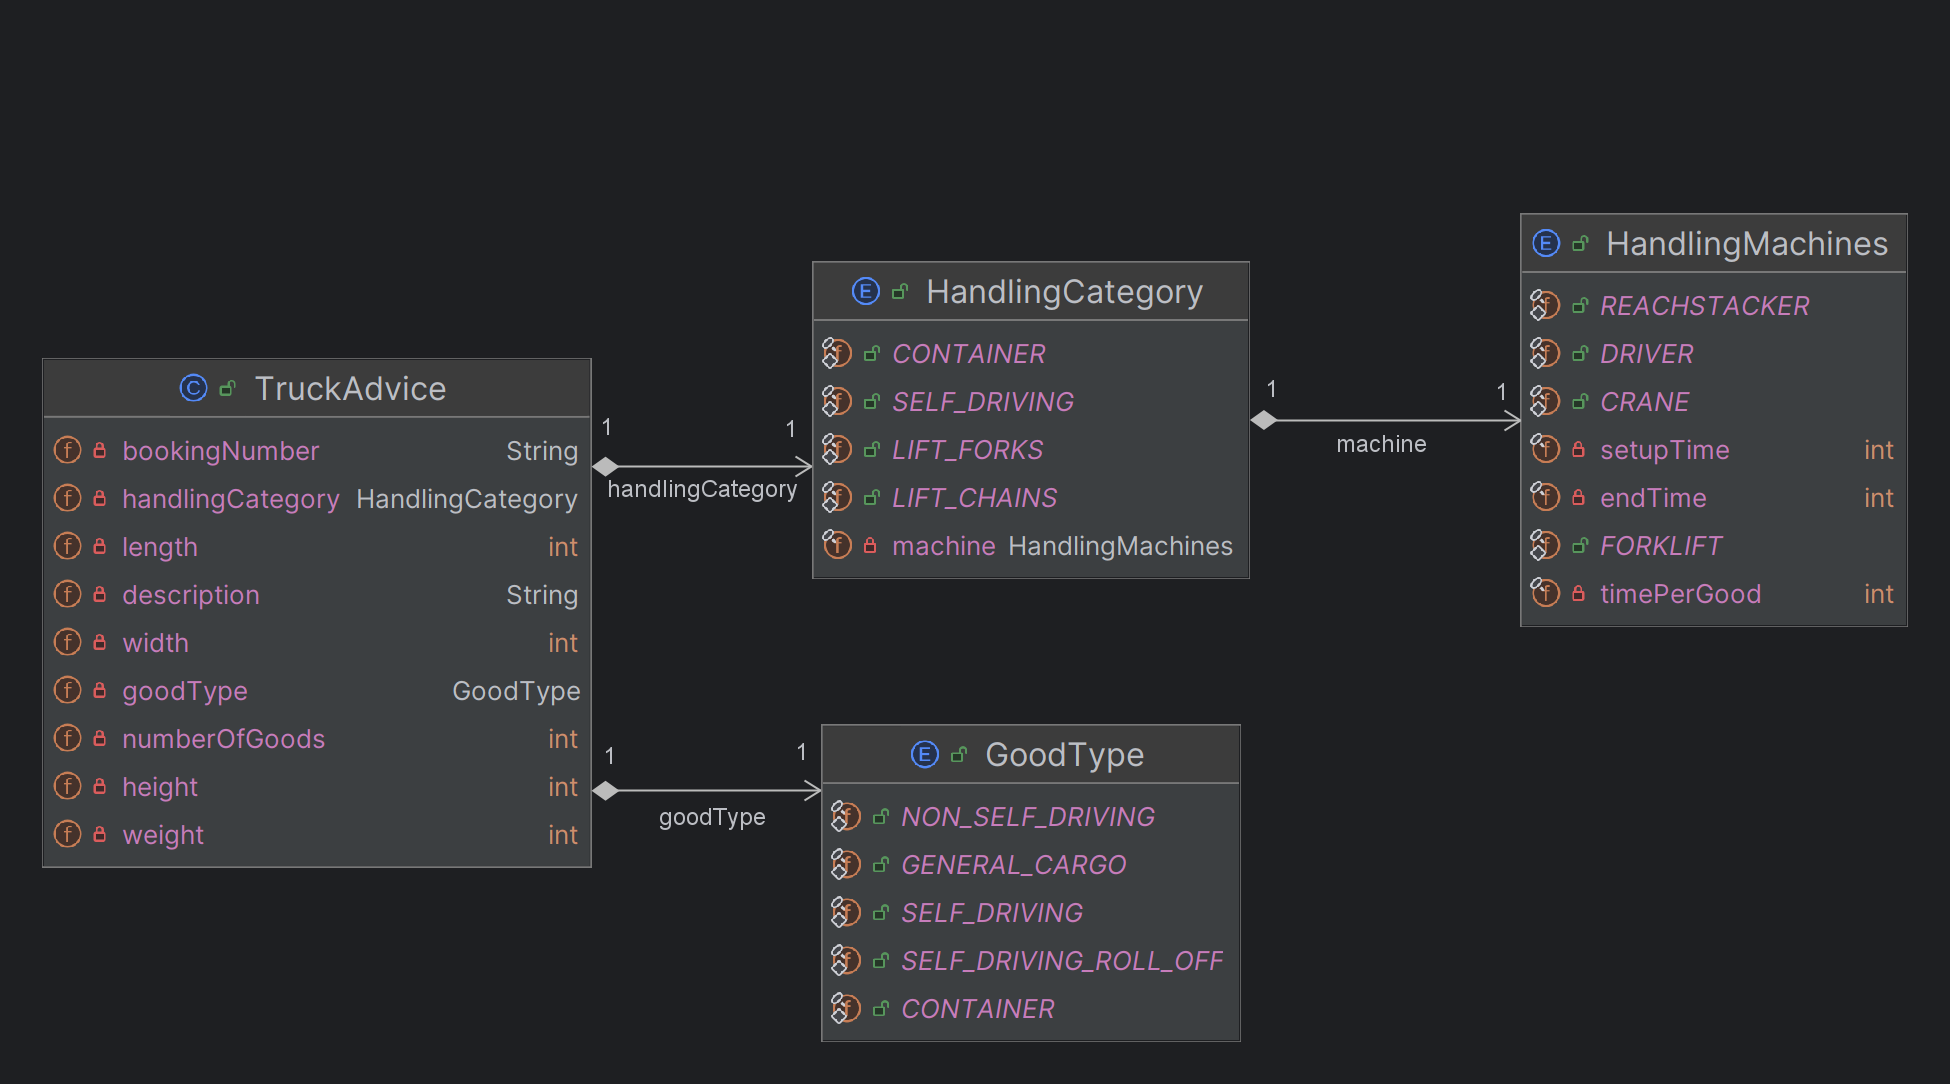
\includegraphics[width=\textwidth]{images/classDiagrams/TSP_TruckAdvice_ClassDiagram.png}
    \caption{Klassendiagramm der Modell-Klassen im Zusammenhang mit TruckAdvice}
    \label{fig:tspClassDiagramTruckAvice}
\end{figure}


Auch hier wurden alle Enums mit Werten entsprechend der Analyse aus Kapitel \ref{sec:analyseAbfertigung} gefüllt. Folgende Werte sind dabei aktuell gesetzt, wobei Erweiterungen durch die Wahl des Typs Enum möglich sind, ohne umfangreichere Anpassungen vornehmen zu müssen: \todo{Enum Werte final?}

GoodType:
\begin{itemize}
    \item CONTAINER
    \item GENERAL\_CARGO
    \item SELF\_DRIVING
    \item SELF\_DRIVING\_ROLL\_OFF
    \item NON\_SELF\_DRIVING
\end{itemize}

HandlingCategory:
\begin{itemize}
    \item LIFT\_CHAINS (HandlingMachine: CRANE)
    \item LIFT\_FORKS (HandlingMachine: FORKLIFT)
    \item SELF\_DRIVING (HandlingMachine: DRIVER)
    \item CONTAINER (HandlingMachine: REACHSTACKER)
\end{itemize}

HandlingMachines:
\begin{itemize}
    \item CRANE(timePerGood: 10, setupTime: 30, endTime: 10)
    \item FORKLIFT(timePerGood: 5, setupTime: 15, endTime: 5)
    \item REACHSTACKER(timePerGood: 3, setupTime: 15, endTime: 10)
    \item DRIVER(timePerGood: 10, setupTime: 5, endTime: 2)
\end{itemize}



\subsubsection{TSP Graph}

Die Besonderheit dieses Algorithmus ist, dass es hier keine bloße Liste von Avisierungen gibt, welche entsprechend geplant werden soll. Es musste in diesem Fall eine Datenstruktur geschaffen werden, welche einen Graphen darstellen und so das TSP repräsentieren kann. Die implementierten Lösungsverfahren sollen dann das so aufbereitete TSP übergeben bekommen und einen optimierten Zeitplan erstellen.

Um diesen Graphen darzustellen, wurde die abstrakte Modell-Klasse \textit{GraphNode} erstellt. Sie dient als Superklasse für alle Knotentypen in diesem Graphen. Ein Knotentyp ist, wie bereits angerissen, die \textit{TruckNode}, welche jeweils eine LKW-Buchung repräsentiert, also die schlussendliche Aufgabe, welche geplant werden soll. Zusätzlich wurde die Klasse \textit{Loader} eingeführt. Sie wird für die Berechnung eines mTSP, also einer Optimierungsaufgabe mit mehreren Ladeplätzen benötigt und ist Teil der Implementierung des in der Planung genannten Verfahrens zur Transformation von mTSP in normale TSP (siehe Kapitel \ref{sec:mstpTransofrmation}). Entscheidende Werte des Graphen sind nun die Kosten an den Kanten zwischen den Knoten. Da es sich hier um einen vollständigen, gerichteten Graphen handeln muss und die Kostenberechnung in dieser Umsetzung dynamisch anhand von Start- und Zielknoten der Kante erfolgt, besitzt jede die \textit{GraphNode} eine Methode zur Kostenberechnung zu einem beliebigen anderen Knoten, welcher dieser Methode übergeben werden kann. So kann der Graph dynamisch gehalten werden, ohne vorab Berechnungen anstellen zu müssen und der Graph selbst kann sehr einfach in einer Liste von die \textit{GraphNode}-Objekten gespeichert werden.

\begin{figure}[H]
    \centering
    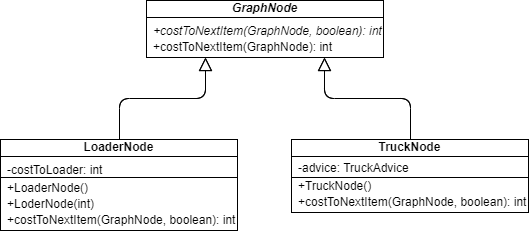
\includegraphics[width=0.8\textwidth]{images/classDiagrams/TSP_Graph_ClassDiagram.png}
    \caption{Klassendiagramm der Modell-Klassen im Zusammenhang mit dem TSP Graphen}
    \label{fig:tspClassDiagramGraph}
\end{figure}


\subsubsection{Zeitplan}

Der Zeitplan selbst, also die Datenstruktur, welche schlussendlich von den TSP Lösungsverfahren erzeugt wird, ist hier einfacher aufgebaut. Sie bietet aber auch hier den großen Vorteil, dass ein über die Algorithmen einheitliches Ausgabeformat erzeugt wird. Ein Zeitplan enthält dabei grundsätzlich zwei Listen: Eine Liste \textit{loaderAdvices}, welche wiederum eine Liste von \textit{TruckAdvices} enthält. Die erste Liste spiegelt dabei die unterschiedlichen Ladeplätze wieder, denen jeweils über die innere Liste eine Menge von Avisierungen zugeordnet ist. Die innere Liste ist dabei nach Reihenfolge der Abfertigung sortiert. Eine zweite, einfache Liste \textit{unscheduled}, welche auch \textit{TruckAdvices} enthält, speichert alle LKW, welche nicht mehr in den Zeitplan gepasst haben.

\begin{figure}[H]
    \centering
    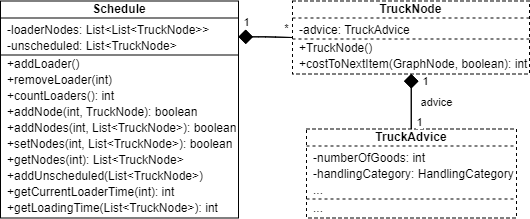
\includegraphics[width=0.8\textwidth]{images/classDiagrams/TSP_Schedule_ClassDiagram.png}
    \caption{Klassendiagramm der Modell-Klassen des Zeitplans}
    \label{fig:tspClassDiagramSchedule}
\end{figure}


\subsubsection{Implementierung von TSP Lösungsverfahren}

\begin{figure}[H]
    \centering
    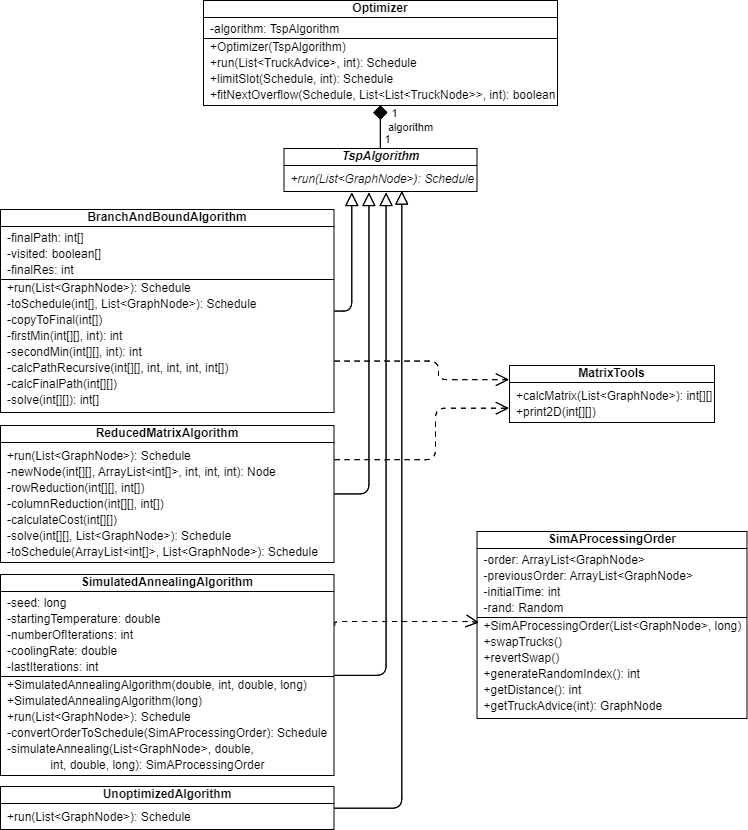
\includegraphics[width=\textwidth]{images/classDiagrams/TSP_Optimizer_ClassDiagram.png}
    \caption{Klassendiagramm der Controller-Klassen zur Lösung des TSP}
    \label{fig:tspClassDiagramOptimizer}
\end{figure}


Um eine einfachere Austauschbarkeit der TSP Verfahren zu erzielen, wurde die \textit{Optimizer} Klasse eingeführt. Sie ermöglicht es, dynamisch eine der zuvor entwickelten Algorithmusklassen zu verwendet. Gleichzeitig können aber über alle Verfahren einheitliche Arbeitsschitte an einer Stelle durchgeführt werden, ohne dass es einer mehrfachen Implementierung bedarf. Zunächst gehört dazu einmal das Auffüllen der Graphen mit den Dummy Ladeplatz-Knoten (also mit \textit{Loader}-Objekten). Die werden in allen TSP Verfahren benötigt, wenn ein mTSP Problem mit mehreren Plätzen vorliegt und kann somit ausgelagert werden. Der \textit{Optimizer} ermöglicht es aber gleichzeitig, eine von außen abstrahierte und vereinfachte Darstellung zu nutzen. Hier wird lediglich eine Liste von \textit{TruckAdvices}, also den Eingaben der LKW Fahrer, benötigt und die Anzahl der verfügbaren Ladeplätze. Die interne Erstellung des Graphen erfolgt dann erst gekapselt in der \textit{Optimizer} Klasse. Der zweite ausgelagerte, da gemeinsame Aspekt, ist das Zuschneiden der optimierten Reihenfolgen auf einen begrenzten Slot. Nachdem die beste Abfertigungsreihenfolge durch die Verfahren gefunden wurde, ist die Überführung in einen Zeitplan prinzipiell nicht kompliziert. Für einen Ladeplatz ist die Reihenfolge bereits fertig und muss nur noch entsprechend zum \textit{Schedule}-Objekt hinzugefügt werden. Für mehrere Ladeplätze müssen die \textit{TruckAdvices} zwischen den \textit{Loader}-Knoten jeweils in eine eigene Teilliste im \textit{Schedule} gespeichert werden. Etwas aufwändiger dagagen ist die Implementierung der in Kapitel \ref{sec:tspToSchedule} geplanten Slotsbegrenzung. Hier war es nötig entsprechende Methoden zu implementieren, welche rekursiv die Überläufe innerhalb der Ladeplätze finden, nach Größe priorisieren und passend geschnitten auf die noch nicht komplett gefüllten Plätze verteilen kann.

Die Implementierung von Lösungsverfahren für das TSP ist der zentrale Teil des Projekts und für die eigentliche Optimierung zuständig. Um eine leichte Austauschbarkeit des genutzten Algorithmus zu erzielen, wurde auch hier eine erweiterbare Implementierung entwickelt, welche die abstrakte Klasse \textit{TspAlgorithm} nutzt. Alle konkreten Implementierungen erben von dieser und können so über eine einheitliche Schnittstelle aufgerufen werden, welche aus einer Liste von \textit{TruckAdvices} und der Anzahl von Ladeplätzen eine bestmögliche Verteilung für ein Zeitplan in Form eines \textit{Schedule} erzeugt. Die Implementierung von passenden Verfahren erwies sich bei genauerer Betrachtung aber als nicht so trivial. Insbesondere, da neben der reinen Implementierung auch eine korrekte Funktionsweise getestet und sichergestellt werden musste. Die folgenden Umsetzungen orientieren sich deshalb an den Java-Implementierungen der Computer Science Education-Plattformen Baeldung \cite{baeldung} und GeeksForGeeks \cite{geeksForGeeks}. Es ließen sich hier auch nach langer Recherche keine anderen Quellen auffinden, welche anwendbare und gleichzeitig im zeitlichen Rahmen dieser Arbeit implementierbare Ansätze boten. Die Qualität und Funkionsfähigkeit der Codes nach einigen kleineren und größeren Anpassungen, wurde dabei durch Tests bei der Implementierung, Prüfungen gegeneinander und auch durch Prüfung der Abläufe mit Hilfe von anderen Quellen (siehe das Kapitel \ref{sec:tspVerfahrenPlanung} zur Planung der Verfahren) sichergestellt. Bei der Implementierung der Verfahren sind einige Besonderheiten und Auffälligkeiten sichtbar geworden, auf welche hier einmal detailliert eingegangen werden soll:

\textbf{Simulated Annealing:} Dieser Algorithmus ist von der Umsetzung und von der Nachvollziehbarkeit her das vergleichsweise einfachste und verständlichste Verfahren. Die Implementierung wurde auf Basis des Beispiels von Baeldung \cite{simABaeldung} umgesetzt. Auf die genaue Funktionsweise wurde bereits in der Konzeption eingegangen. Die Eingangsparameter sind hier sehr einfach, gearbeitet wird zunächst einmal direkt mit der Datenstruktur des Graphen, wie sie zuvor beschrieben wurde. Um die Reihenfolge und die Tauschoperationen leichter abbilden zu können, wurde die Klasse \textit{SimAProcessingOrder} eingeführt. Hier wird Simulated Annealing mit dem zufälligen Tausch von zwei Knoten des Graphen durchgeführt. Die Klasse erlaubt es diese Tauschoperationen auf einer temporären Kopie des Eingangsgraphen durchzuführen und kann gleichzeitig auch den letzten Tausch rückgängig machen, falls dies gewünscht ist. Ein besonderer Schritt dieses Verfahrens ist es, dass über Schleifen ein Abkühlungsprozess nachgebildet wird. Dieser Prozess folgt einigen Parametern, hauptsächlich Starttemperatur, Abkühlungsrate und Anzahl von Iterationen. Das Festlegen dieser Parameter ist eine Herausforderung und hängt von vielen Faktoren, unter anderem auch der Art der Eingangswerte des Algorithmus ab. Aus diesem Grund wurde die Bestimmung und Bewertung der besten Werte in das Kapitel Evaluation dieser Arbeit ausgelagert, dort werden entsprechende Tests konzipiert und im ergebnis die besten Parameter in diese Klasse als Standardwerte eingefügt. Abschließend muss das interne \textit{SimAProcessingOrder}-Objekt noch in ein allgemeingültiges \textit{Schedule}-Objekt umgewandelt werden. Da dies ein teils spezifischer Vorgang ist, der sich von dem der anderen Algorithmen unterscheidet, wurde dies auch noch als direkter Teil der \textit{SimulatedAnnealingAlgorithm} Klasse implementiert.% Schon bei der Implementierung auf, dass es bei Ausführung dieses Algorithmus gewisse Grenzen gibt, wenn der Eingangsgraph größer wird. Dies betrifft hier gar nicht so sehr die Ausführungsdauer, viel mehr kommt die Größe des Arbeitsspeichers an seine Grenzen. Eine genauere Betrachtung mit praxisbezogenen Daten soll auch hier in der Evaluation stattfinden.

\textbf{Branch and Bound:} Die Besonderheit dieser Implementierung ist, dass sie auf Basis einer Kostenmatrix arbeitet. Um den Implementierungsaufwand geringer zu halten und um die fertige Implementierung von GeeksForGeeks \cite{geeksForGeeksBnB} in Teilen Nutzen zu können, wurde zunächst eine Methode entwickelt, welche die Graph-Datenstruktur in eine Matrix aus Integer-Werten überführen kann. Da die Kosten bereits als Berechnungsschritte in der Graphen-Implementierung vorhanden waren, ist dies aber sehr einfach möglich, indem über Schleifen einmal jede Kombination vorgerechnet und in einem zweidimensionalen Array gespeichert wird. Da diese Matrix auch im Reduced Matrix Verfahren gebraucht wird, wurde die entsprechende Methode in die eigene Klasse \textit{MatrixTools} ausgelagert. Da das eigentliche Finden des kürzesten Weges wie erwähnt nicht ganz trivial ist, wurden alle nun folgenden Lösungs-Methoden weitgehend aus dem Implementierungsbeispiel übernommen. Schlussendlich muss nun nur noch eine Methode zur Überführung in das bekannte \textit{Schedule}-Objekt erfolgen. Bei diesem Verfahren fielen schon bei ersten Tests in der Implementierung Grenzen auf, die Ausführungszeit ist ein limitierender Faktor. Es werden schnell extrem hohe Rechenzeiten erreicht, welche mit dem Hinzufügen einzelner Knoten exponentiell ansteigen, sodass schon mit sehr wenigen Knoten Ausführungszeiten erreicht werden, welche auch über einige Stunden und somit den sinnvoll nutzbaren Rahmen hinaus gehen. Hier folgt eine genauere Auswertung im Kapitel Evaluation dieser Arbeit.

\textbf{Reduced Matrix:} Das dritte Lösungsverfahren nutzt, wie der Name Reduced Matrix Verfahren auch schon vermuten lässt, ebenfalls eine Kostenmatrix als Eingangsformat. Die entsprechende Berechnungsmethode wurde schon für das Branch and Bound Verfahren entwickelt und kann hier wieder genutzt werden. Die danach benötigten Methoden zur Reduzierung und Berechnung des kürzesten Pfades wurden ebenfalls weitgehend aus dem Beispiel von GeeksForGeeks \cite{geeksForGeeksRm} übernommen. Auch hier wäre eine komplette Eigenentwicklung sehr komplex und fehlerträchtig. Deshalb wurde die spezielle Lösung genutzt und am Ende erneut eine Überführung der internen Darstellung des Algorithmus in ein allgemeines \textit{Schedule}-Objekt vorgenommen. Bei der Ausführung hat sich auch in diesem Verfahren schnell gezeigt, dass die mögliche Größe der lösbaren Graphen sehr begrenzt ist. Hier liegt der limitierende Faktor allerdings bei der Größe des verfügbaren Arbeitsspeichers, der vermutlich durch eine große Zahl von gespeicherten Matrizen sehr schnell ausgenutzt wird. Eine genauere Evaluation der Grenzen folgt auch hier zusammen mit der Auswertung der anderen Verfahren.

\textbf{Unoptimized:} Dies ist die Umsetzung des in Kapitel \ref{sec:konzeptTspVergleichswerte} beschriebenen und geplanten Ansatzes zur Generierung von Vergleichswerten. Auch in diesem Projekt wurde die Implementierung als weitere Subklasse des allgemeinen \textit{TspAlgorithm} durchgeführt. Es handelt sich hier zwar nicht um ein direktes Lösungsverfahren, es kann so auch Nutzen aus der Modularität ziehen. So können auf gleichem Weg für identische Eingangsdaten neben den optimierten Werten auch Vergleichswerte für den potentiellen unoptimierten Fall berechnet werden. Auch die Ausgangsdaten sind somit im identischen Format und lassen sich so direkt miteinander vergleichen.

Insgesamt ist zu den Algorithmen und deren Implementierung anzumerken, dass deren Hauptzweck ist, einen Eindruck davon zu bekommen, dass der Optimierungsansatz über das TSP valide ist und zu guten Lösungen führt. Es sollten hier auch Verfahren auf deren Vor- und Nachteilen, sowie auf deren Verwendbarkeit für das hier vorliegende Szenario untersucht werden. Es hat sich aber auch gezeigt, dass eine Umsetzung durchaus sehr komplex und nicht einfach ist. Insbesondere gute und optimierte Verfahren, welche schnell die beste Lösung liefern, sind nicht einfach umzusetzen und deshalb auch ein Problem, mit welchem sich die Informatik schon sein Jahrzehnten beschäftigt \cite{travelingSalesman}. Aus diesem Grund ist es auf jeden Fall ein Erfolg, dass hier zumindest auf den ersten Blick zielführende Lösungen gefunden wurden, dennoch kann sicherlich mit deutlich mehr Aufwand ein besseres Verfahren gefunden werden. Durch die modulare Implementation sollte dies aber auch gut ersetzbar sein.


\subsubsection{Analyse der Zeitplanungen}

Um einen späteren, einheitlichen Vergleich der TSP Lösungsverfahren durchführen zu können, wurde auch hier eine eigene Controller-Klasse \textit{ScheduleAnalyser} erstellt. Diese kann aus den zuvor erstellten Zeitplänen interessante Werte und Metriken errechnen, welche dann in den folgenden Auswertungen genutzt werden.

\begin{figure}[H]
    \centering
    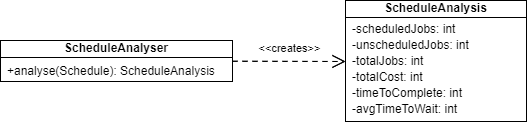
\includegraphics[width=0.9\textwidth]{images/classDiagrams/TSP_ScheduleAnalyser_ClassDiagram.png}
    \caption{Klassendiagramm von ScheduleAnalyser und der erzeugten ScheduleAnalysis}
    \label{fig:tspClassDiagramScheduleAnalyser}
\end{figure}

Da bei diesem Algorithmus der Fokus und das Optimierungsziel etwas anders gesetzt wurde, sind hier auch einige andere Werte interessant. Folgende Zahlen werden in diesem Fall jeweils berechnet:

\begin{itemize}
    \item \textit{scheduledJobs:} Die Anzahl der LKW, die erfolgreich in den Zeitslot eingeplant werden konnten. Da die Erhöhung dieses Wertes immer noch ziel der gesamten Optimierung ist, aber nicht direktes dies des TSP-Verfahrens, ist das Verhalten dieses Wertes für die Auswertung besonders interessant.
    \item \textit{unscheduledJobs:} Die Anzahl von LKW, die zeitlich nicht mehr in den Slot gepasst haben.
    \item \textit{totalJobs:} Die Gesamtanzahl der avisierten LKW, welche versucht wurden, auf den Slot zu verteilen (entspricht scheduledJobs+unscheduledJobs).
    \item \textit{totalCost:} Die Gesamtkosten bzw. die Gesamtzeit zur Abarbeitung des gesamten Zeitplans. Dies ist die Variable nach der das TSP optimiert wird.
    \item \textit{timeToComplete:} Die Dauer vom Beginn des Slots, bis alle LKW abgefertigt sind.
    \item \textit{avgTimeToWait:} Durchschnittliche Wartezeit, von Beginn des Slots bis zum Beginn der Abfertigung aller LKW.
\end{itemize}


\subsubsection{JUnit Tests}

Für das Testen und Bewerten der zuvor entwickelten Algorithmen, sollen auch für dieses Projekt JUnit Test genutzt werden. Die genauen Testfälle und deren Implementierung werden auch hier erst im Kapitel Evaluation beschrieben und erstellt. Die Tests sollen dabei aber sehr ähnlich zu denen im anderen Projekt sein und nutzen deshalb sehr ähnliche, testübergreifend entwickelte Klassen als wiederverwendbare Grundlage. Die Test-Klasse \textit{AdviceGenerator} kann auch hier dafür genutzt werden, zufällige aber realitätsnahe Eingangsdatensätze für die Testfälle zu erzeugen. Der \textit{CsvExporter} wurde auch weitgehend identisch aus dem anderen Projekt übernommen und erlaubt auch für die hier entwickelten Tests eine einfache und einheitliche Speicherung der Testergebnisse im CSV Format, um sie anschließend mit R-Skripten auswerten zu können.